\documentclass[../tex_main/NEMO_manual]{subfiles}
\begin{document}
% ================================================================
% Chapter ---�� Miscellaneous Topics
% ================================================================
\chapter{Miscellaneous Topics}
\label{chap:MISC}
\minitoc

\newpage
$\ $\newline    % force a new ligne

% ================================================================
% Representation of Unresolved Straits
% ================================================================
\section{Representation of unresolved straits}
\label{sec:MISC_strait}

In climate modeling, it often occurs that a crucial connections between water masses
is broken as the grid mesh is too coarse to resolve narrow straits. For example, coarse 
grid spacing typically closes off the Mediterranean from the Atlantic at the Strait of 
Gibraltar. In this case, it is important for climate models to include the effects of salty 
water entering the Atlantic from the Mediterranean. Likewise, it is important for the 
Mediterranean to replenish its supply of water from the Atlantic to balance the net 
evaporation occurring over the Mediterranean region. This problem occurs even in 
eddy permitting simulations. For example, in ORCA 1/4\deg several straits of the Indonesian 
archipelago (Ombai, Lombok...) are much narrow than even a single ocean grid-point.

We describe briefly here the three methods that can be used in \NEMO to handle 
such improperly resolved straits. The first two consist of opening the strait by hand 
while ensuring that the mass exchanges through the strait are not too large by 
either artificially reducing the surface of the strait grid-cells or, locally increasing 
the lateral friction. In the third one, the strait is closed but exchanges of mass, 
heat and salt across the land are allowed.
Note that such modifications are so specific to a given configuration that no attempt 
has been made to set them in a generic way. However, examples of how 
they can be set up is given in the ORCA 2\deg and 0.5\deg configurations. For example, 
for details of implementation in ORCA2, search: 
\texttt{ IF( cp\_cfg == "orca" .AND. jp\_cfg == 2 ) }

% -------------------------------------------------------------------------------------------------------------
%       Hand made geometry changes
% -------------------------------------------------------------------------------------------------------------
\subsection{Hand made geometry changes}
\label{subsec:MISC_strait_hand}

$\bullet$ reduced scale factor in the cross-strait direction to a value in better agreement 
with the true mean width of the strait. (\autoref{fig:MISC_strait_hand}).
This technique is sometime called "partially open face" or "partially closed cells".
The key issue here is only to reduce the faces of $T$-cell ($i.e.$ change the value 
of the horizontal scale factors at $u$- or $v$-point) but not the volume of the $T$-cell.
Indeed, reducing the volume of strait $T$-cell can easily produce a numerical 
instability at that grid point that would require a reduction of the model time step.
The changes associated with strait management are done in \mdl{domhgr}, 
just after the definition or reading of the horizontal scale factors. 

$\bullet$ increase of the viscous boundary layer thickness by local increase of the 
fmask value at the coast (\autoref{fig:MISC_strait_hand}). This is done in 
\mdl{dommsk} together with the setting of the coastal value of fmask 
(see  \autoref{sec:LBC_coast})

%>>>>>>>>>>>>>>>>>>>>>>>>>>>>
\begin{figure}[!tbp] 	 \begin{center}
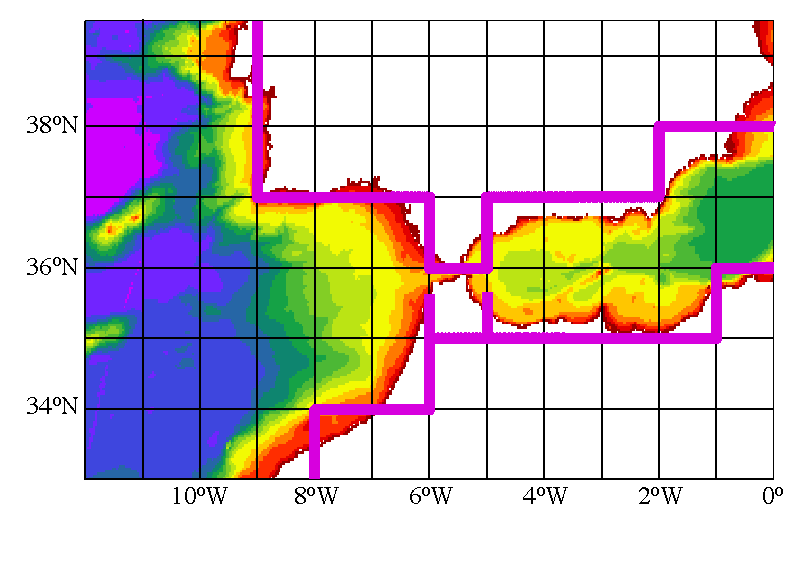
\includegraphics[width=0.80\textwidth]{Fig_Gibraltar}
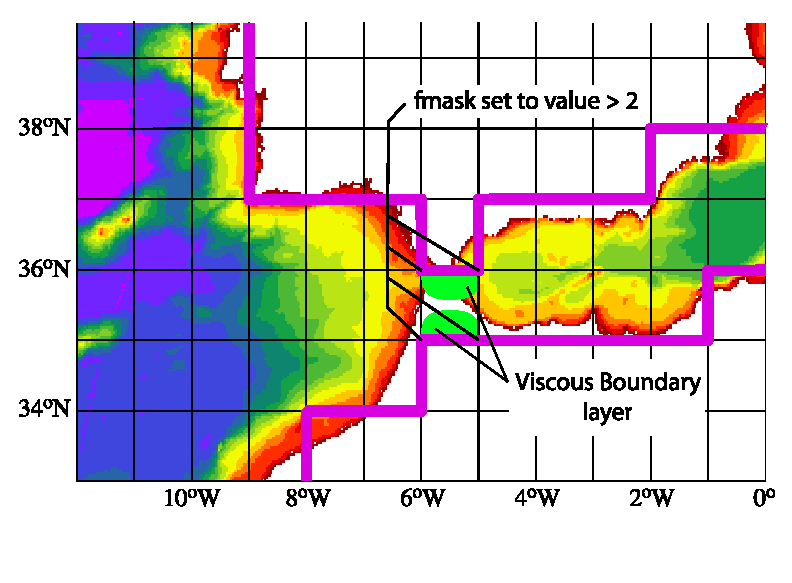
\includegraphics[width=0.80\textwidth]{Fig_Gibraltar2}
\caption{	\protect\label{fig:MISC_strait_hand} 
Example of the Gibraltar strait defined in a $1^{\circ} \times 1^{\circ}$ mesh. 
\textit{Top}: using partially open cells. The meridional scale factor at $v$-point 
is reduced on both sides of the strait to account for the real width of the strait 
(about 20 km). Note that the scale factors of the strait $T$-point remains unchanged. 
\textit{Bottom}: using viscous boundary layers. The four fmask parameters 
along the strait coastlines are set to a value larger than 4, $i.e.$ "strong" no-slip 
case (see \autoref{fig:LBC_shlat}) creating a large viscous boundary layer 
that allows a reduced transport through the strait.}
\end{center}   \end{figure}
%>>>>>>>>>>>>>>>>>>>>>>>>>>>>


% ================================================================
% Closed seas
% ================================================================
\section{Closed seas (\protect\mdl{closea})}
\label{sec:MISC_closea}

\colorbox{yellow}{Add here a short description of the way closed seas are managed}


% ================================================================
% Sub-Domain Functionality 
% ================================================================
\section{Sub-domain functionality}
\label{sec:MISC_zoom}

\subsection{Simple subsetting of input files via NetCDF attributes}

The extended grids for use with the under-shelf ice cavities will result in redundant rows
around Antarctica if the ice cavities are not active. A simple mechanism for subsetting
input files associated with the extended domains has been implemented to avoid the need to
maintain different sets of input fields for use with or without active ice cavities. The
existing 'zoom' options are overly complex for this task and marked for deletion anyway.
This alternative subsetting operates for the j-direction only and works by optionally
looking for and using a global file attribute (named: \np{open\_ocean\_jstart}) to
determine the starting j-row for input. The use of this option is best explained with an
example: Consider an ORCA1 configuration using the extended grid bathymetry and coordinate
files:
\vspace{-10pt}
\ifile{eORCA1\_bathymetry\_v2}
\ifile{eORCA1\_coordinates}
\noindent These files define a horizontal domain of 362x332. Assuming the first row with
open ocean wet points in the non-isf bathymetry for this set is row 42 (Fortran indexing)
then the formally correct setting for \np{open\_ocean\_jstart} is 41. Using this value as the
first row to be read will result in a 362x292 domain which is the same size as the original
ORCA1 domain. Thus the extended coordinates and bathymetry files can be used with all the
original input files for ORCA1 if the ice cavities are not active (\np{ln\_isfcav =
.false.}). Full instructions for achieving this are:

\noindent Add the new attribute to any input files requiring a j-row offset, i.e:
\vspace{-10pt}
\begin{cmds}
ncatted  -a open_ocean_jstart,global,a,d,41 eORCA1_coordinates.nc 
ncatted  -a open_ocean_jstart,global,a,d,41 eORCA1_bathymetry_v2.nc
\end{cmds}
 
\noindent Add the logical switch to \ngn{namcfg} in the configuration namelist and set true:
%--------------------------------------------namcfg--------------------------------------------------------
\forfile{../namelists/namcfg}
%--------------------------------------------------------------------------------------------------------------

\noindent Note the j-size of the global domain is the (extended j-size minus
\np{open\_ocean\_jstart} + 1 ) and this must match the size of all datasets other than
bathymetry and coordinates currently. However the option can be extended to any global, 2D
and 3D, netcdf, input field by adding the:
\vspace{-10pt}
\begin{forlines}
lrowattr=ln_use_jattr
\end{forlines}
optional argument to the appropriate \np{iom\_get} call and the \np{open\_ocean\_jstart} attribute to the corresponding input files. It remains the users responsibility to set \np{jpjdta} and \np{jpjglo} values in the \np{namelist\_cfg} file according to their needs.

%>>>>>>>>>>>>>>>>>>>>>>>>>>>>
\begin{figure}[!ht] 	  \begin{center}
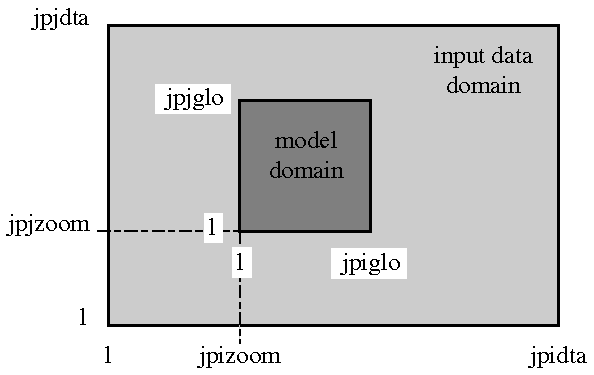
\includegraphics[width=0.90\textwidth]{Fig_LBC_zoom}
\caption{	\protect\label{fig:LBC_zoom}
Position of a model domain compared to the data input domain when the zoom functionality is used.}
\end{center}   \end{figure}
%>>>>>>>>>>>>>>>>>>>>>>>>>>>>


% ================================================================
% Accuracy and Reproducibility
% ================================================================
\section{Accuracy and reproducibility (\protect\mdl{lib\_fortran})}
\label{sec:MISC_fortran}

\subsection{Issues with intrinsinc SIGN function (\protect\key{nosignedzero})}
\label{subsec:MISC_sign}

The SIGN(A, B) is the \textsc {Fortran} intrinsic function delivers the magnitude 
of A with the sign of B. For example, SIGN(-3.0,2.0) has the value 3.0.
The problematic case is when the second argument is zero, because, on platforms 
that support IEEE arithmetic, zero is actually a signed number. 
There is a positive zero and a negative zero.

In \textsc{Fortran}~90, the processor was required always to deliver a positive result for SIGN(A, B) 
if B was zero. Nevertheless, in \textsc{Fortran}~95, the processor is allowed to do the correct thing 
and deliver ABS(A) when B is a positive zero and -ABS(A) when B is a negative zero. 
This change in the specification becomes apparent only when B is of type real, and is zero, 
and the processor is capable of distinguishing between positive and negative zero, 
and B is negative real zero. Then SIGN delivers a negative result where, under \textsc{Fortran}~90 
rules,  it used to return a positive result. 
This change may be especially sensitive for the ice model, so we overwrite the intrinsinc 
function with our own function simply performing :   \\
\verb?   IF( B >= 0.e0 ) THEN   ;   SIGN(A,B) = ABS(A)  ?    \\
\verb?   ELSE                   ;   SIGN(A,B) =-ABS(A)     ?  \\
\verb?   ENDIF    ? \\
This feature can be found in \mdl{lib\_fortran} module and is effective when \key{nosignedzero}
is defined. We use a CPP key as the overwritting of a intrinsic function can present 
performance issues with some computers/compilers.


\subsection{MPP reproducibility}
\label{subsec:MISC_glosum}

The numerical reproducibility of simulations on distributed memory parallel computers 
is a critical issue. In particular, within NEMO global summation of distributed arrays 
is most susceptible to rounding errors, and their propagation and accumulation cause 
uncertainty in final simulation reproducibility on different numbers of processors.
To avoid so, based on \citet{He_Ding_JSC01} review of different technics, 
we use a so called self-compensated summation method. The idea is to estimate 
the roundoff error, store it in a buffer, and then add it back in the next addition. 

Suppose we need to calculate $b = a_1 + a_2 + a_3$. The following algorithm 
will allow to split the sum in two ($sum_1 = a_{1} + a_{2}$ and $b = sum_2 = sum_1 + a_3$) 
with exactly the same rounding errors as the sum performed all at once.
\begin{align*}
	sum_1 \ \  &= a_1 + a_2 \\
	error_1     &= a_2 + ( a_1 - sum_1 ) \\
	sum_2 \ \  &= sum_1 + a_3 + error_1 \\
	error_2     &= a_3 + error_1 + ( sum_1 - sum_2 ) \\
	b \qquad \ &= sum_2 \\
\end{align*}
An example of this feature can be found in \mdl{lib\_fortran} module.
It is systematicallt used in glob\_sum function (summation over the entire basin excluding 
duplicated rows and columns due to cyclic or north fold boundary condition as well as 
overlap MPP areas). The self-compensated summation method should be used in all summation
in i- and/or j-direction. See \mdl{closea} module for an example.
Note also that this implementation may be sensitive to the optimization level. 

\subsection{MPP scalability}
\label{subsec:MISC_mppsca}

The default method of communicating values across the north-fold in distributed memory applications
(\key{mpp\_mpi}) uses a \textsc{MPI\_ALLGATHER} function to exchange values from each processing
region in the northern row with every other processing region in the northern row. This enables a
global width array containing the top 4 rows to be collated on every northern row processor and then
folded with a simple algorithm. Although conceptually simple, this "All to All" communication will
hamper performance scalability for large numbers of northern row processors. From version 3.4
onwards an alternative method is available which only performs direct "Peer to Peer" communications
between each processor and its immediate "neighbours" across the fold line. This is achieved by
using the default \textsc{MPI\_ALLGATHER} method during initialisation to help identify the "active"
neighbours. Stored lists of these neighbours are then used in all subsequent north-fold exchanges to
restrict exchanges to those between associated regions. The collated global width array for each
region is thus only partially filled but is guaranteed to be set at all the locations actually
required by each individual for the fold operation. This alternative method should give identical
results to the default \textsc{ALLGATHER} method and is recommended for large values of \np{jpni}.
The new method is activated by setting \np{ln\_nnogather} to be true ({\bf nammpp}). The
reproducibility of results using the two methods should be confirmed for each new, non-reference
configuration.

% ================================================================
% Model optimisation, Control Print and Benchmark
% ================================================================
\section{Model optimisation, control print and benchmark}
\label{sec:MISC_opt}
%--------------------------------------------namctl-------------------------------------------------------
\forfile{../namelists/namctl} 
%--------------------------------------------------------------------------------------------------------------

 \gmcomment{why not make these bullets into subsections?}
Options are defined through the  \ngn{namctl} namelist variables.

$\bullet$ Vector optimisation:

\key{vectopt\_loop} enables the internal loops to collapse. This is very 
a very efficient way to increase the length of vector calculations and thus 
to speed up the model on vector computers.
 
% Add here also one word on NPROMA technique that has been found useless, since compiler have made significant progress during the last decade.
 
% Add also one word on NEC specific optimisation (Novercheck option for example)
 
$\bullet$ Control print %: describe here 4 things:

1- \np{ln\_ctl} : compute and print the trends averaged over the interior domain 
in all TRA, DYN, LDF and ZDF modules. This option is very helpful when 
diagnosing the origin of an undesired change in model results. 

2- also \np{ln\_ctl} but using the nictl and njctl namelist parameters to check 
the source of differences between mono and multi processor runs.

%%gm   to be removed both here and in the code
3- last digit comparison (\np{nn\_bit\_cmp}). In an MPP simulation, the computation of 
a sum over the whole domain is performed as the summation over all processors of 
each of their sums over their interior domains. This double sum never gives exactly 
the same result as a single sum over the whole domain, due to truncation differences. 
The "bit comparison" option has been introduced in order to be able to check that 
mono-processor and multi-processor runs give exactly the same results. 
%THIS is to be updated with the mpp_sum_glo  introduced in v3.3
% nn_bit_cmp  today only check that the nn_cla = 0 (no cross land advection)
%%gm end

$\bullet$  Benchmark (\np{nn\_bench}). This option defines a benchmark run based on 
a GYRE configuration (see \autoref{sec:CFG_gyre}) in which the resolution remains the same 
whatever the domain size. This allows a very large model domain to be used, just by 
changing the domain size (\jp{jpiglo}, \jp{jpjglo}) and without adjusting either the time-step 
or the physical parameterisations. 

% ================================================================
\end{document}




